\newpage
\subsection{Attività preliminari di avvio ed analisi dei requisiti}
Il periodo preliminare di analisi si svolge dal 15/11/2018 al 14/01/2019 e partono dalla formazione del gruppo terminando poi alla prima milestone ovvero la consegna dei documenti. \newline
Le attività principali sono le seguenti:
\begin{itemize}
	\item\textbf{Norme di progetto:} questo è il primo documento poiché contiene tutte le norme atte a regolare internamente il gruppo Dream Corp. che spaziano dall'indentatura del codice alle regole per stendere i documenti stessi;
	\item\textbf{Studio di fattibilità:} redatta dagli Analisti questa è un' attività bloccante per l'inizio dell'analisi dei requisiti. Consiste in un analisi dei pro e dei contro dei vari capitolati con il fine di una scelta ponderata del capitolato;
	\item\textbf{Analisi dei requisiti:} dopo aver scelto il capitolato è necessario approfondire i requisiti richiesti dalla proponente. Svolto ancora una volta dagli Analisti;
	\item\textbf{Piano di progetto:} questa attività è bloccante per la stesura della lettera di presentazione. Viene svolta dal Responsabile che ha lo scopo di analizzare le attività necessarie e la loro scadenza al fine di garantire la  buona riuscita del progetto mentre L'amministratore analizza i rischi nei quali il gruppo Dream Corp. può incombere durate il percorso. Inoltre in questa attività vengono stabilite le risorse disponibili per l'intero progetto;
	\item\textbf{Piano di qualifica:} in questa attività viene redatto il documento \textit{Piano di Qualifica} che ha lo scopo di individuare dei metodi per garantire la qualità del prodotto;
	\item\textbf{Glossario:} questa attività consiste nella redazione del \textit{Glossario}, dove verranno inseriti tutti i termini considerati possibilmente ambigui;
	\item\textbf{Lettera di presentazione:} attività che consiste nello studio autonomo di ogni membro del gruppo e, soprattutto, nella preparazione del materiale di supporto per la stesura della \textit{Lettera di presentazione} necessaria per il gruppo al fine di essere scelto come fornitore.
\end{itemize}

\begin{figure}[!htpb]
	\centering
	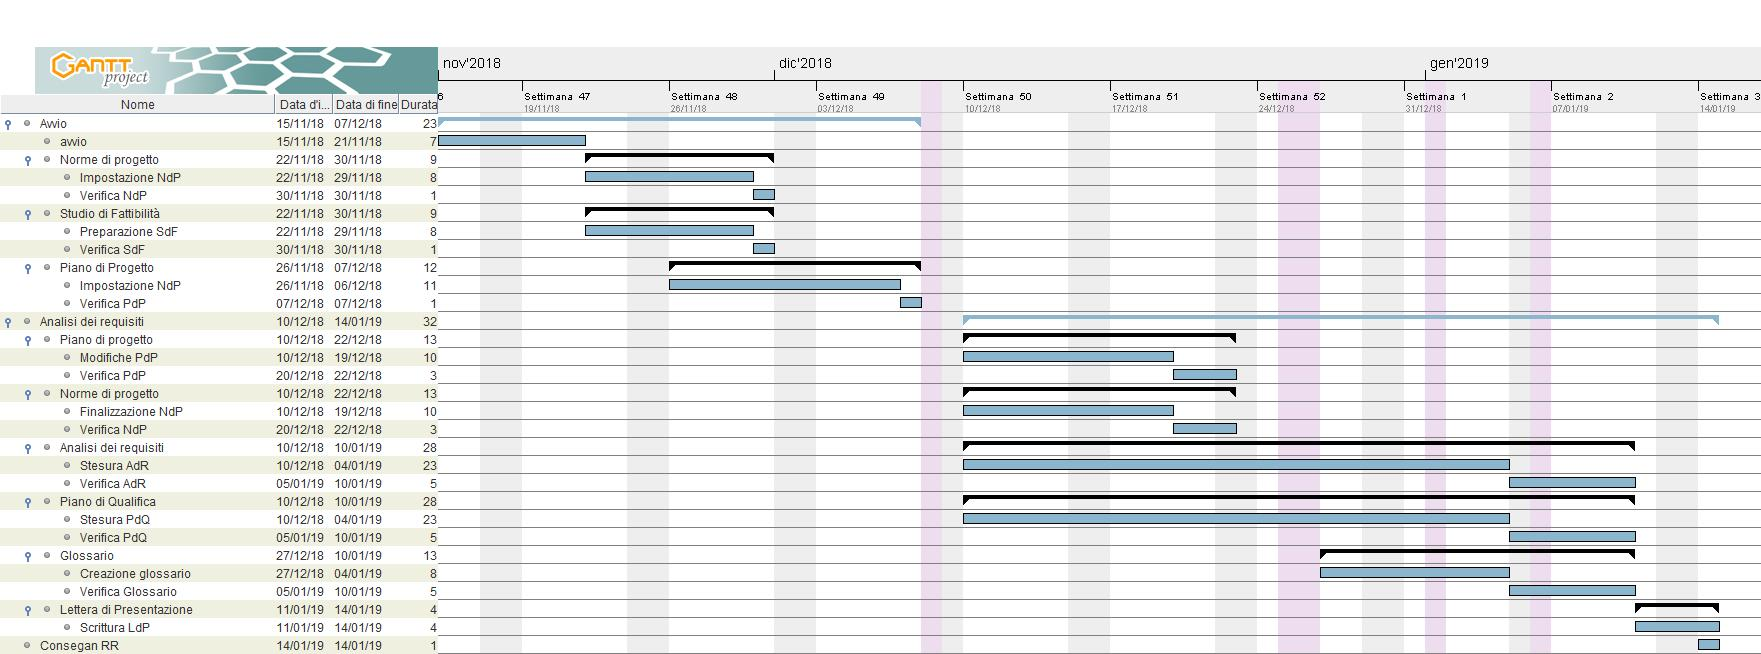
\includegraphics[width=\textwidth]{Gantt_prima_fase.jpg}
	\caption{Diagramma di Gantt del periodo di Analisi}
\end{figure}

\begin{figure}[!htpb]
\centering
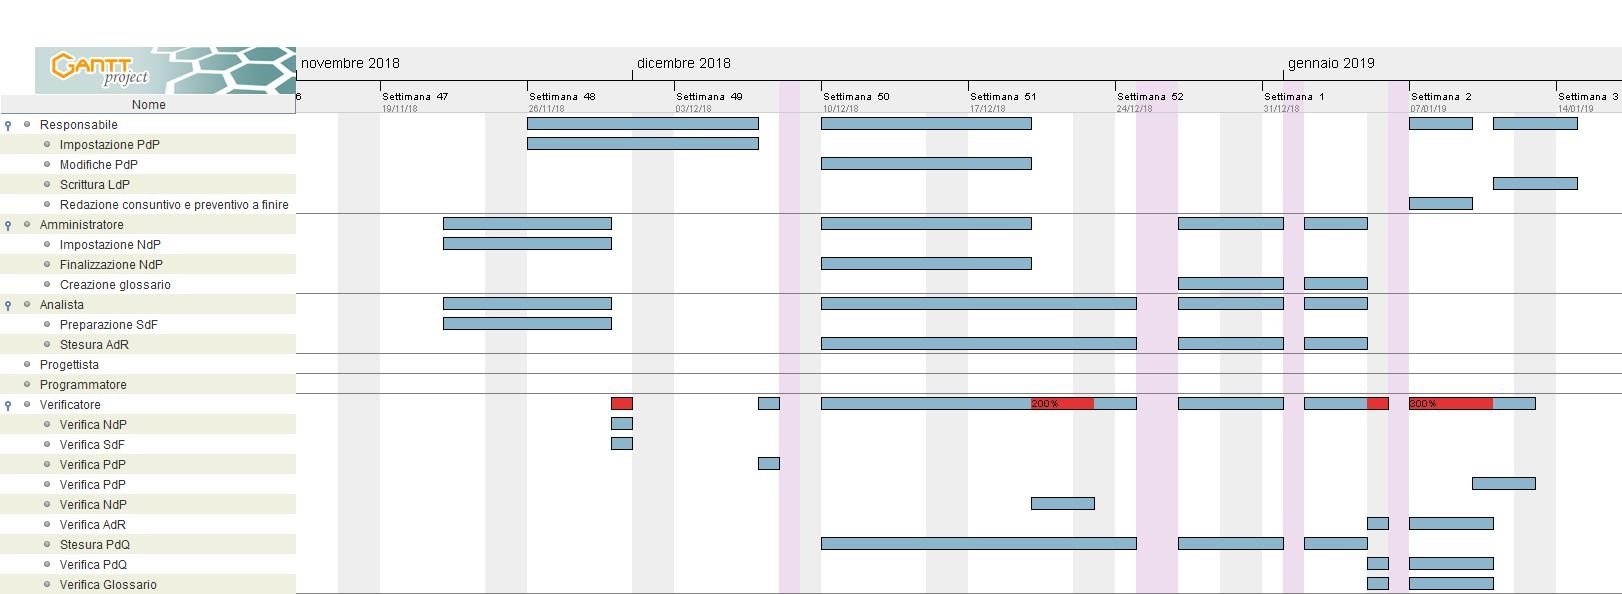
\includegraphics[width=\textwidth]{Gantt_prima_fase_risorse.jpg}
\caption{Diagramma di Gantt delle risorse del periodo di Analisi}
\end{figure}

\begin{table}[!htpb]
	\centering
	\renewcommand{\arraystretch}{2} 
	\rowcolors{2}{gray!25}{white}
	\begin{tabular}{|c|p{4.5cm}|p{4.5cm}|}
		\rowcolor{orange!50}
		\hline
		\multicolumn{3}{|c|}{\textbf{Suddivisione temporale}}\\
		\hline
		\textbf{Ruolo} & \textbf{15/11/18 - 10/12/18} & \textbf{11/12/18 - 14/01/19} \\
		\hline
		\textbf{Responsabile} & \daG & \pie \\
		\hline
		\textbf{Amministratore} &\parbox{4.5cm}{\gia \\ \mat} & \mar\\
		\hline
		\textbf{Analista} & \parbox{4.5cm}{\pie \\ \mic} & \parbox{4.5cm}{\daG \\ \daL \\ \mat} \\
		\hline
		\textbf{Progettista} & - & - \\
		\hline
		\textbf{Programmatore} & - & - \\
		\hline
		\textbf{Verificatore} & \parbox{4.5cm}{\daL \\ \mar} & \parbox{4.5cm}{\mic \\ \gia} \\
		\hline
	\end{tabular}
	\caption{Suddivisione temporale del periodo di Analisi}
\end{table}
